\documentclass[border=4pt]{standalone}
\usepackage{tikz}
\usetikzlibrary{arrows,arrows.spaced}
\begin{document}
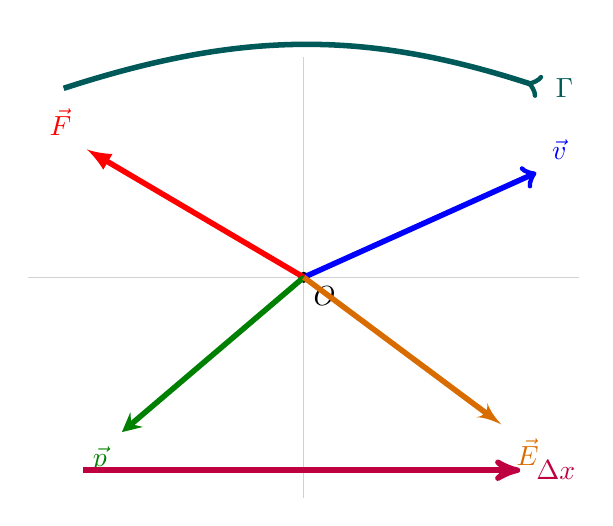
\begin{tikzpicture}
  \draw[gray!35] (-3.5,0) -- (3.5,0);
  \draw[gray!35] (0,-2.8) -- (0,2.8);
  \fill (0,0) circle (2pt) node[below right] {$O$};

  \draw[blue,line width=2pt,-{spaced to}] (0,0) -- (3,1.35) node[above right] {$\vec v$};
  \draw[red,line width=2pt,-{spaced latex}] (0,0) -- (-2.8,1.65) node[above left] {$\vec F$};
  \draw[green!50!black,line width=2pt,-{spaced stealth}] (0,0) -- (-2.35,-2) node[below left] {$\vec p$};
  \draw[orange!85!black,line width=2pt,-{spaced latex'}] (0,0) -- (2.55,-1.9) node[below right] {$\vec E$};
  \draw[purple,line width=2pt,-{spaced stealth'}] (-2.8,-2.45) -- (2.8,-2.45) node[right] {$\Delta x$};
  \draw[teal!70!black,line width=2pt,-{spaced to reversed}] (-3.05,2.4) to[bend left=18] (3.05,2.4) node[right] {$\Gamma$};
\end{tikzpicture}
\end{document}
